% !TEX root = main.tex
\chapter{Redes Neurais Artificiais}
\label{cha:ann}


A história de \textbf{Redes Neurais Artificiais} começou em 1943 com a fundação do modelo matemático proposto em \citep{mcculloch1943logical}, que em 1951 permitiu abordagens inspiradas na biologia cerebral e por aplicações em inteligência artificial \citep{kleene1951representation}, como no caso da criação de \textbf{Perceptron}\footnote{A menor unidade de processamento de uma rede neural, que pode fazer pequenos trabalhos de processamento por si só, mas pode cooperar com outros para alcançar uma convergência, mesmo para um trabalho enorme distribuído por um grande número de neurônios trabalhando em uma rede.} \citep{rosenblatt1958perceptron}, um algoritmo de classificação binária baseado no aprendizado supervisionado, um dos desenvolvimentos mais importantes no campo, publicado em 1958. Outro grande passo foi dado em 1967, quando foi publicado um trabalho sobre redes envolvendo múltiplas camadas \citep{ivakhnenko1967cybernetics}. A Seção \ref{sec:ann_perceptron} esclarecerá o funcionamento do Perceptron, então a Seção \ref{sec:ann_arch_and_prop} trará explicações sobre arquitetura e propriedades das redes neurais.

Alguns anos mais tarde, mais precisamente em 1972, dois grandes problemas foram identificados nos modelos de redes neurais então conhecidos: a incapacidade dos perceptrons básicos para processar operações de ``ou exclusivo'' (XOR) e a escassez de poder computacional exigido para se trabalhar com redes neurais de muitas camadas \citep{minsky1972perceptrons}. Estes problemas dificultaram muito para que houvesse qualquer avanço relevante nesta área durante vários anos, mas em 1975 foi proposto o \textbf{Backpropagation} \citep{werbos1975beyond}, um novo algoritmo que faria esta área de pesquisa continuar a ser interessante, uma vez que resolveria o problema de operação XOR e aceleraria o processamento em redes multi-camadas ajustando os pesos das camadas por meio de uma distribuição de erro. Uma explicação detalhada sobre Backpropagation será oferecida na Seção \ref{sec:ann_backpropagation}.

Considerando a alta demanda de poder computacional que tais modelos trouxeram consigo, pode-se dizer que muitos avanços na área foram conquistados nos anos seguintes, também por conta de trabalhos envolvendo paralelismo, por exemplo. \citep{rumelhart1986psychological}, de 1986. Em 1993 algumas melhorias foram alcançadas em redes neurais \citep{180705}; e, em 2010, o uso de Unidades de Processamento Gráfico na paralelização desta tarefa \citep{scherer2010evaluation} foi extremamente importante.

Também em 2006, um modelo de representações de alto nível foi proposto usando camadas sucessivas de variáveis latentes com máquinas Boltzmann \citep{hinton2006fast}. E, ainda mais recentemente, em 2013, foi introduzida uma rede suficientemente avançada para reconhecer conceitos avançados, como gatos em vídeos do YouTube \citep{le2013building} de maneira não supervisionada. Essas implementações de um grande número de camadas passaram a incluir em sua nomenclatura o termo ``Deep'' e, portanto, o termo \textbf{Deep Learning} tornou-se popular quando se refere a redes neurais artificiais profundas, também chamadas \textbf{Deep Neural Networks}.

Atualmente, existem inúmeras aplicações de Deep Learning para as mais diversas áreas de atividade, como neurociências \citep{Varatharajan2018}, IoT (Internet das Coisas) \citep{8396317}, segurança redes de computadores \citep{8291134}, reconhecimento facial \citep{8253595}, instrumentação \citep{8319916}, telecomunicações \citep{8359094}, imageamento médico \citep{8359121}, detecção de objetos \citep{8253582} tratamento de distúrbios da voz \citep{8337897}, mobilidade \citep{8344803} e tantos outros.



%   ----------------------
%   ----- Perceptron -----
%   ----------------------
\section{Perceptron}
\label{sec:ann_perceptron}

O \textit{Perceptron} é compreendido como a menor unidade neural capaz de realizar a tarefa de classificar dados linearmente separáveis, separando-os através de uma região fronteiriça denominada hiperplano\footnote{Hiperplano nada mais é do que a generalização de um plano para dimensões superiores; trata-se de uma forma geométrica com uma dimensão a menos que o hiperespaço, que é o caso que utiliza-se de todas as dimensões disponíveis}. O perceptron foi desenvolvido por Frank Rosenblatt \citep{rosenblatt1958perceptron}, enquanto trabalhava no \textit{Cornell Aeronautical Laboratory}, em um projeto financiado pelo \textit{Office of Naval Research}; e, diferentemente do que hoje se esperaria, teria sido originalmente planejado para ser uma máquina, não um programa de computador.

Em seu próprio trabalho original, Rosenblatt exibiu um esboço de como ele compreendia ser a organização do \textit{Perceptron}, bem como suas intraconexões, que envolviam componentes que ele chamou de Retina, Área de Projeção, Área de Associação e Respostas, como exibido na Figura \ref{fig:ann_perceptron_organization}.

\begin{figure}[H]
    \centering
    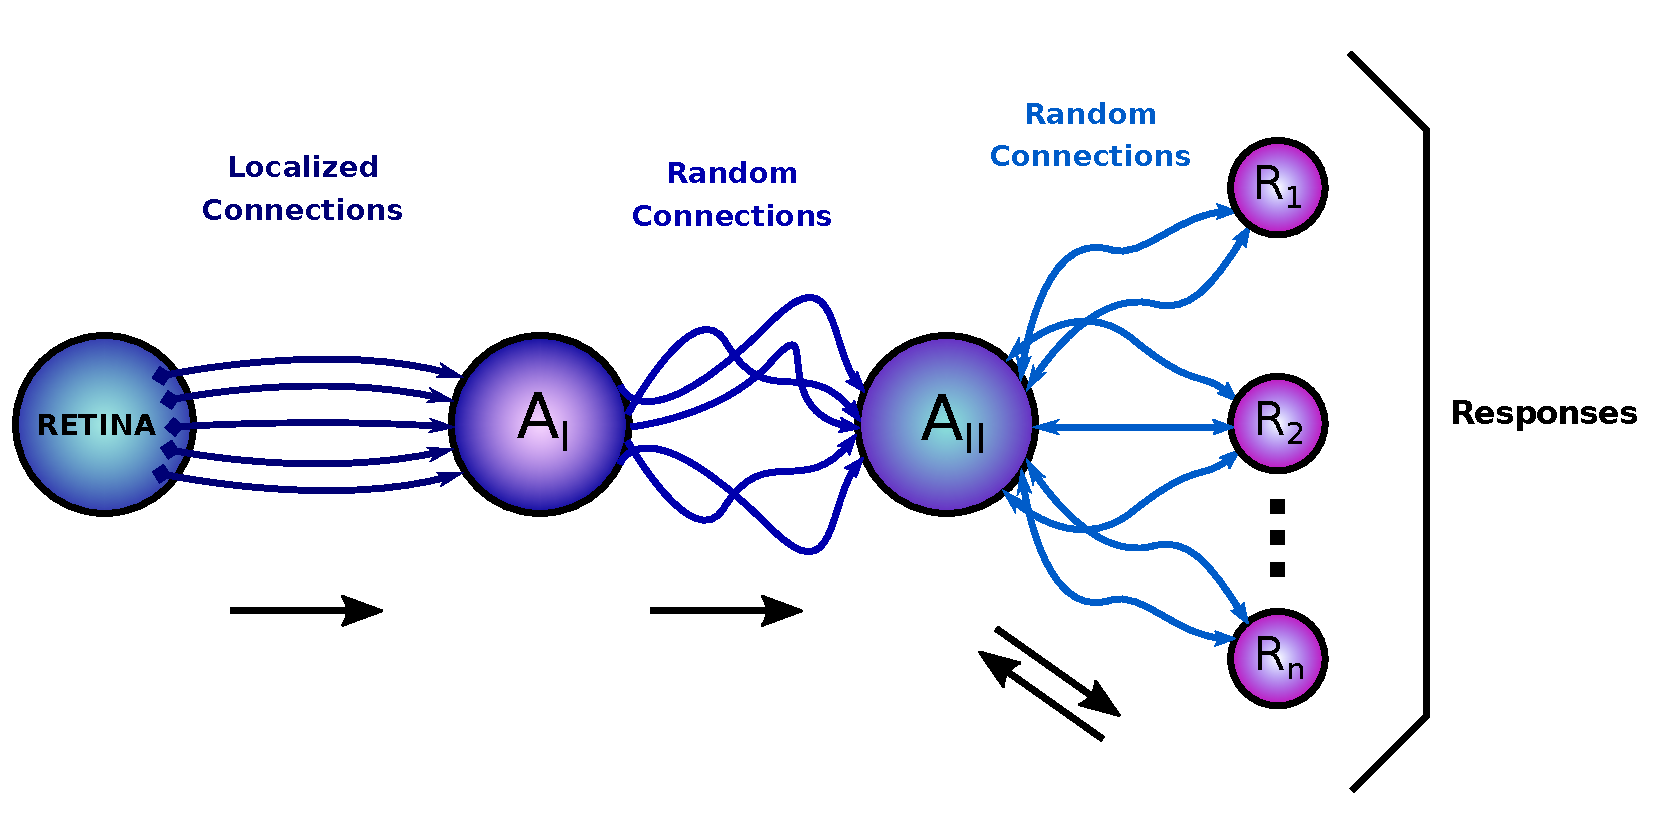
\includegraphics[width=0.85\textwidth]{figs/ann_perceptron_original_organization.pdf}
    \caption{Organização de um \textit{Perceptron}, segundo \citep{rosenblatt1958perceptron}.}
    \label{fig:ann_perceptron_organization}
\end{figure}

A Retina trata-se do primeiro componente dessa arquitetura; e é composta por unidades sensoriais com um comportamento que Rosenblatt assumiu como sendo \textit{tudo ou nada}, que pode ser mapeado binariamente. Os impulsos coletados pelos sensores da retina são enviados às chamadas \textit{células de associação}, que se localizam na \textit{área de projeção} (representada na Figura \ref{fig:ann_perceptron_organization} pela região circular $A_{I}$), mas essa região não está presente em todos os modelos de organização; no caso de não estar presente, a conexão é feita de forma direta entre os sensores da retina e a \textit{área de associação} ($A_{II}$).

As unidades da \textit{área de projeção} podem receber estímulos oriundos dos sensores da retina que resultem em excitação ou em inibição. O próprio conceito por detrás do que é comumente chamado de \textit{função de ativação} foi trazido neste mesmo trabalho, dado que, segundo Rosenblatt, as unidades $A$ emitem uma saída\footnote{Para os propósitos de seu modelo, Rosenblatt considerou a saída como sendo unitária, embora reconheça a possibilidade de ser utilizada outra abordagem.} sempre que a soma de todas as entradas da unidade em questão resultar em um valor igual ou superior ao limiar $\theta$ definido. As conexões feitas entre as unidades da área de projeção ($A_{I}$) e as da área de associação ($A_{II}$) foram tratadas como aleatórias, assim sendo, apesar de haver conexões entre unidades das diferentes áreas, tais conexões não necessariamente respeitarão uma específica distribuição; além disso, vale ressaltar que as características e os comportamentos das unidades em si, independentemente de a qual região pertençam, são os mesmos.

A respeito das \textit{respostas} ($R_{1}, \dots, R_{n}$), que são descritas como células ou grupos de células, seu comportamento é similar ao das unidades $A$; suas conexões, contudo, são um tanto diferentes, dado que, apesar de também serem feitas aleatoriamente, são altamente numerosas e são bidirecionais, permitindo uma comunicação diferenciadas com as unidades da área de associação ($A_{II}$), havendo para cada resposta $R$ um \textit{conjunto de origem}\footnote{Em uma tradução livre do que originalmente fora chamado de \textit{source-set}.}, ou seja, um conjunto de unidades $A_{II}$ que façam conexão com o a resposta em questão. A comunicação bidirecional permite a existência de \textit{feedback} da resposta para as unidades $A_{II}$ com as quais se comunica; e podem ser (a) excitatórias para todas as células de seu conjunto de origem ou (b) inibitórias para todas as células que não transmitam para a resposta em questão.

A partir de uma perspectiva mais contemporânea, o Perceptron passou a ser retratado de uma forma menos abstrata, utilizando funções algébricas explícitas e bem definidas, o que justifica, inclusive, a utilização de uma ilustração mais objetiva, assim como a representada pela Figura \ref{fig:ann_perceptron_new_organization}. Mas vale lembrar que esta nova versão é apenas uma forma diferente de representar artisticamente a mesma estrutura organizacional concebita por Rosenblatt. Não se trata, portanto, de uma real mudança da arquitetura original; apenas é feita uma ilustração que acompanhe uma interpretação sutilmente mais convidativa a partir de um olhar da perspectiva computacional.

\begin{figure}[H]
    \centering
    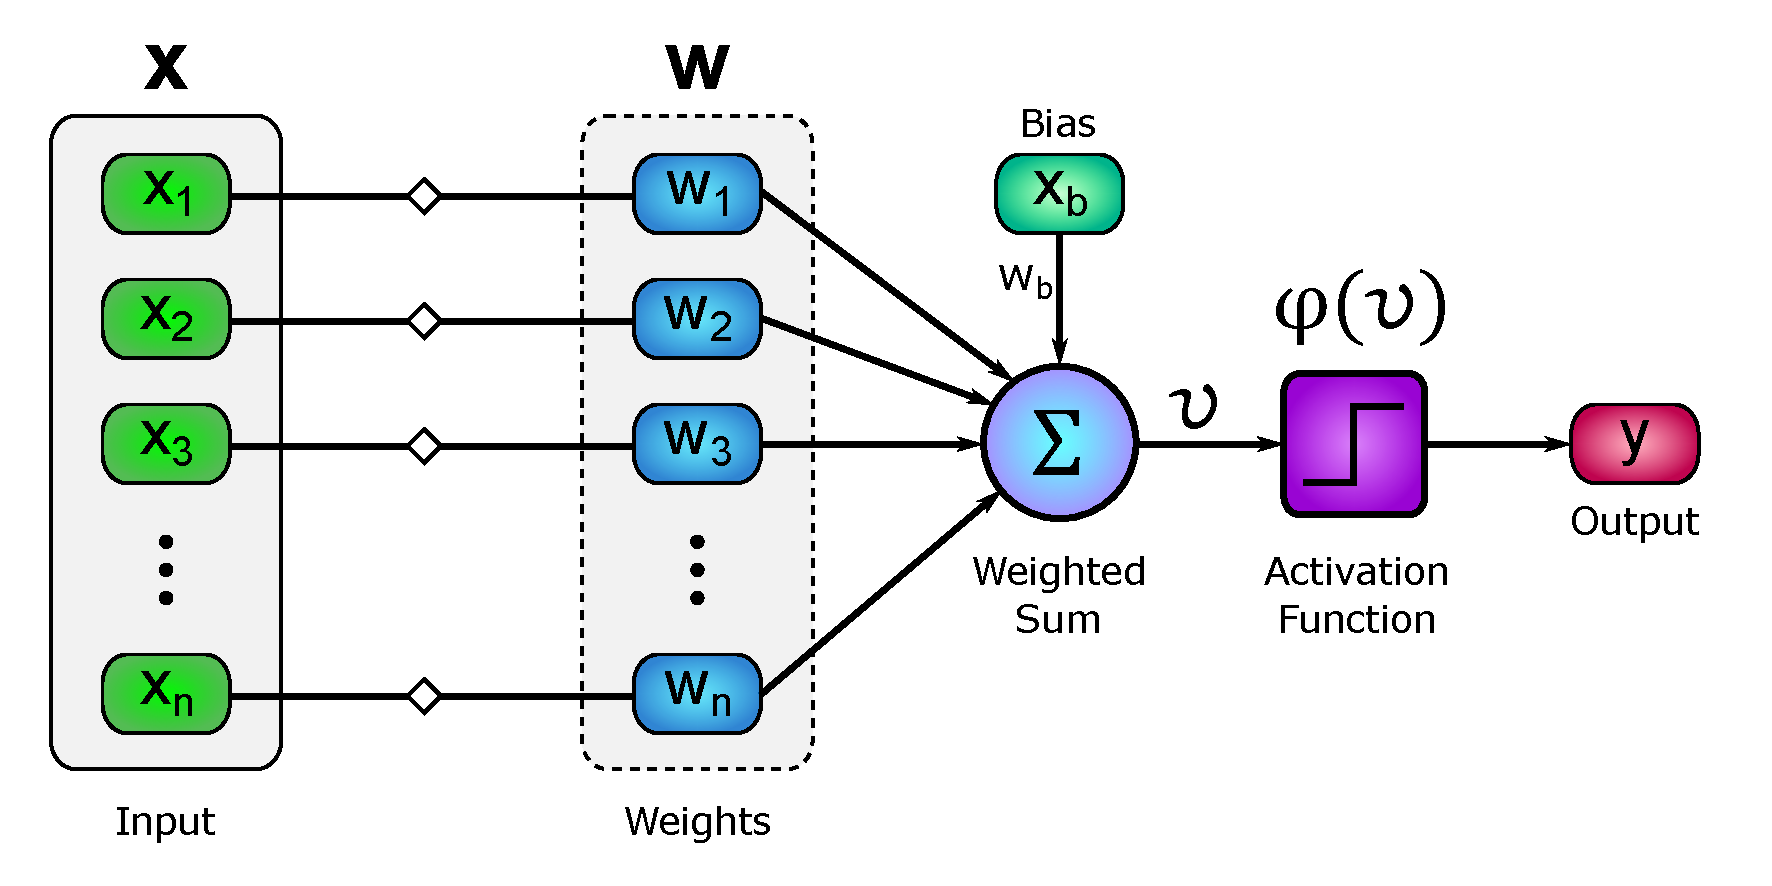
\includegraphics[width=1.00\textwidth]{figs/ann_perceptron_new_organization.pdf}
    \caption{Representação contemporânea da arquitetura de um \textit{Perceptron}.}
    \label{fig:ann_perceptron_new_organization}
\end{figure}


A partir da Figura \ref{fig:ann_perceptron_new_organization}, pode-se compreender que há um conjunto de entradas, $\bm{x}$, respectivamente ponderadas por um conjunto de pesos, $\bm{w}$, que, junto a um \textit{bias}, são somadas, então o resultado dessa soma é utilizado como entrada de uma \textit{função de ativação}, responsável por emitir o valor da saída, $\bm{y}$. O somatório utiliza-se de uma combinação linear causada pela soma ponderada das entradas, além do \textit{bias}, o que resulta na separação de duas regiões por um \textit{hiperplano} \citep{haykin1999neural}, cuja definição matemática é dada por

\begin{equation}
    \sum_{i=1}^{N} w_{i} x_{i} + b = 0
    \label{eq:ann_perceptron_hyperplane}
    \hspace{0.1cm},
    \vspace{0.2cm}
\end{equation}

\noindent onde $N$ representa o número total de entradas\footnote{O trabalho original de Rosenblatt considerava um arranjo matricial em formato 20x20 em que cada unidade consistia em um sensor fotovoltaico que lia um sinal luminoso e emitia uma resposta de 0 ou 1 quando lia um cartão.} e, portanto, também de seus respectivos pesos para que seja possível efetuar as ponderações; e $b$ representa o \textit{bias}. A partir do resultado do somatório, chega-se à \textit{função de ativação}, a respeito da qual será melhor discutido na seção seguinte.



%   ----- Funções de Ativação -----
\section{Funções de Ativação}
\label{sec:ann_activation_functions}

Um dos elementos mais importantes que compõem um \textit{Perceptron} é a \textit{função de ativação}, que funciona como um filtro que auxilia na tomada de decisões sobre o que fazer com o sinal resultante dos estímulos individuais que a ele chegam, sendo um dos responsáveis finais pela saída a ser obtida. Existem muitos tipos distintos de funções de ativação, não havendo uma função sequer que necessariamente seja melhor que todas as demais em todos os cenários possíveis, o que significa que sempre deverá ser analisado o cenário em questão, quais são os valores possíveis de entrada, quais as saídas desejadas e, também, qual o comportamento da função em toda a região intermediária, afinal, não são apenas os extremos que interferem no desempenho da rede; todos os elementos interferem, embora haja os que possam interferir em maior intensidade.

Uma das funções mais simples é a função \textit{identidade}, que permite quaisquer valores de entrada e saída, mas não se trata de uma das funções mais exploradas contemporaneamente; em vez disso, a função que assume tal posição de prestígio é a função ReLU, que será trazida ainda neste mesmo capítulo. Como o foco deste projeto não são as funções de ativação \textit{per se}, não será feita uma discussão aprofundada quanto a qualquer uma das funções, contudo, a fim de fornecer um material que possa ser utilizado pelo leitor para visualizar mais facilmente os efeitos de algumas funções de ativação, foram selecionadas algumas das mais comumente exploradas para que sejam aqui matematicamente definidas e tenham seu comportamento exibido graficamente para diferentes valores de \textit{bias}.


\begin{definition}[Função Identidade]
    Dada uma entrada $x$, a função Identidade pode ser definida como:

    \begin{equation}
        f[x] = x
        \vspace{0.2cm}
        \label{eq:ann_identity_function}
    \end{equation}

    A derivada da função identidade é:

    \begin{equation}
        f'[x] = 1
        \label{eq:ann_identity_function_dy}
    \end{equation}
    
\end{definition}

A Figura \ref{fig:ann_identity_function} exibe o comportamento da função identidade, bem com o de sua primeira derivada.

\begin{figure}[H]
    \centering
    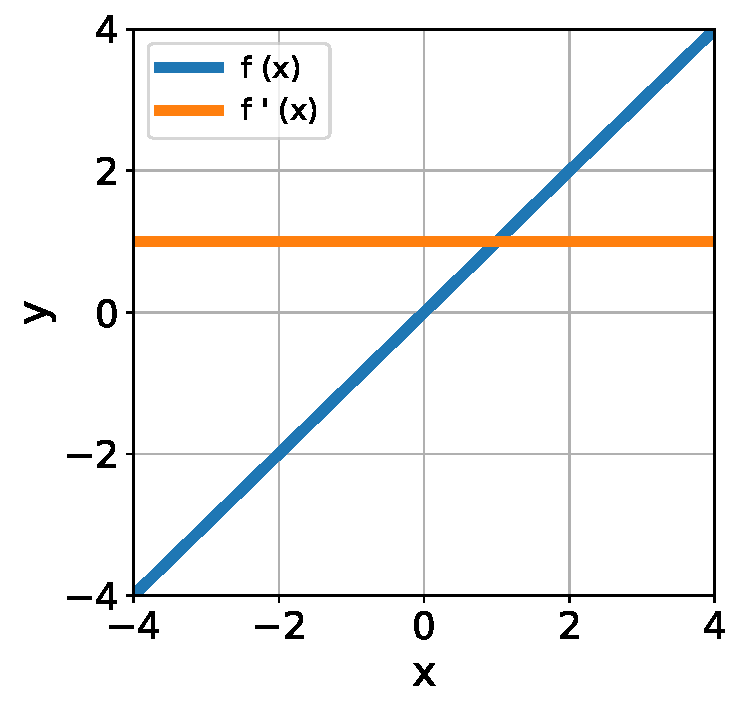
\includegraphics[width=0.65\textwidth]{figs/ann_identity_function.pdf}
    \caption{Comportamento da função identidade.}
    \label{fig:ann_identity_function}
\end{figure}


\linebreak
\newpage


\begin{definition}[Função Degrau Unitário]
    Dada uma entrada $x$, a função Degrau Unitário, também chamada de função Degrau Binário, pode ser definida como:

    \begin{equation}
        f[x] = u[x] = 
        \begin{cases}
            0, & \text{se $x < 0$}\\
            1, & \text{se $x \geq 0$}
        \end{cases}
        \vspace{0.2cm}
        \label{eq:ann_step_function}
    \end{equation}

    A derivada da função degrau unitário é:

    \begin{equation}
        f'[x] = u[x] = 
        \begin{cases}
            0, & \text{se $x \neq 0$}\\
            \text{?}, & \text{se $x = 0$}
        \end{cases}
        \vspace{0.2cm}
        \label{eq:ann_step_function_dy}
    \end{equation}
    
\end{definition}

A Figura \ref{fig:ann_step_function} exibe o comportamento da função degrau unitário (ou binário) e sua primeira derivada.

\begin{figure}[H]
    \centering
    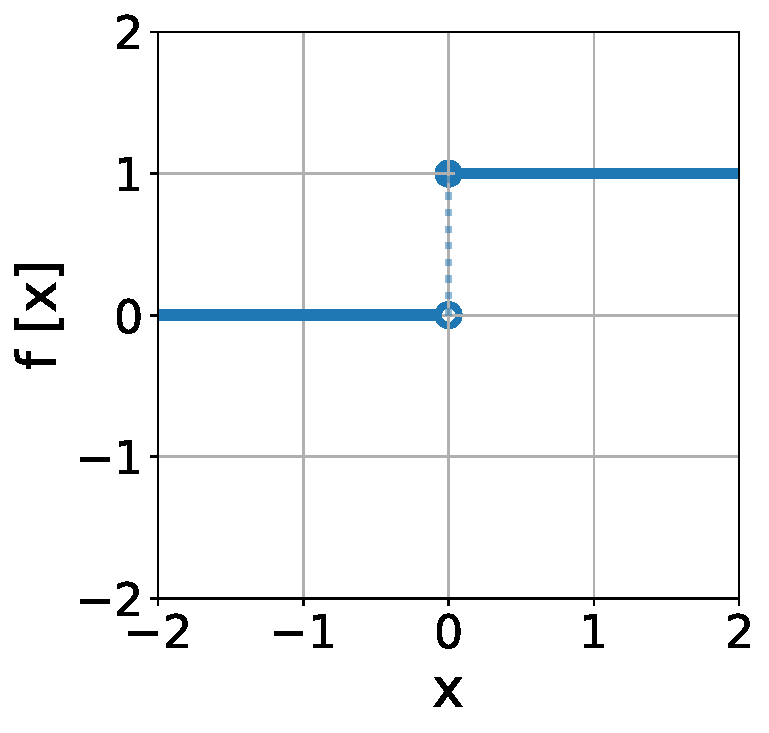
\includegraphics[width=0.65\textwidth]{figs/ann_unit_step_function.pdf}
    \caption{Comportamento da função degrau unitário.}
    \label{fig:ann_step_function}
\end{figure}


\linebreak
\newpage


\begin{definition}[Função Logística]
    Dada uma entrada $x$, a função Logística pode ser definida como:

    \begin{equation}
        f[x] = \sigma [x] = \dfrac{1}{1 + e^{-x}}
        \vspace{0.2cm}
        \label{eq:ann_logistic_function}
    \end{equation}

    A derivada da função logística é:

    \begin{equation}
        f'[x] = f[x]\ (1 - f[x])
        \label{eq:ann_logistic_function_dy}
    \end{equation}
    
\end{definition}

A Figura \ref{fig:ann_logistic_function} exibe o comportamento da função logística.

\begin{figure}[H]
    \centering
    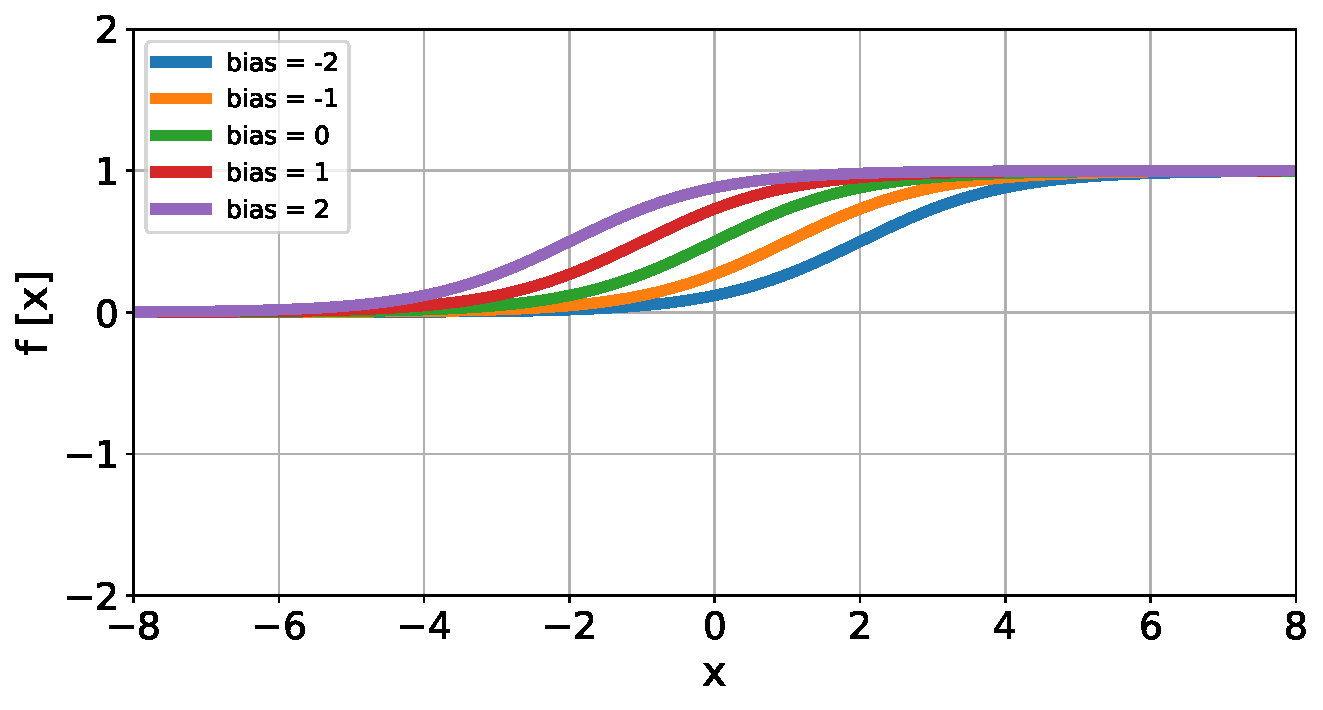
\includegraphics[width=0.65\textwidth]{figs/ann_logistic_function.pdf}

    \caption{Comportamento da função logística.}
    \label{fig:ann_logistic_function}
\end{figure}


\linebreak
\newpage


\begin{definition}[Função Tangente Hiperbólica]
    Dada uma entrada $x$, a função Tangente Hiperbólica pode ser definida como:

    \begin{equation}
        f[x] = \text{tanh}(x) = \dfrac{e^{x} - e^{-x}}{e^{x} + e^{-x}}
        \vspace{0.2cm}
        \label{eq:ann_tanh_function}
    \end{equation}

    A derivada da função tangente hiperbólica é:

    \begin{equation}
        f'[x] = 1 - (f[x])^{2}
        \label{eq:ann_tanh_function_dy}
    \end{equation}

\end{definition}

A Figura \ref{fig:ann_tanh_function} exibe o comportamento da função tangente hiperbólica e de sua derivada.

\begin{figure}[H]
    \centering
    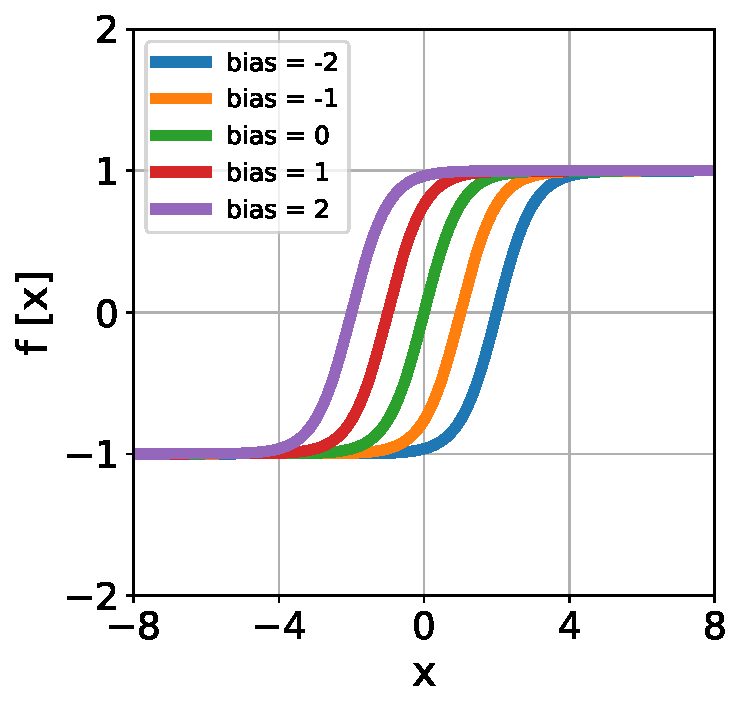
\includegraphics[width=0.65\textwidth]{figs/ann_tanh_function.pdf}

    \caption{Plot da função tangente hiperbólica.}
    \label{fig:ann_tanh_function}
\end{figure}


\linebreak
\newpage


\begin{definition}[Função Arco Tangente]
    Dada uma entrada $x$, a função Arco Tangente pode ser definida como:

    \begin{equation}
        f[x] = \text{tan}^{-1}(x)
        \vspace{0.2cm}
        \label{eq:ann_arctan_function}
    \end{equation}

    A derivada da função arco tangente é:

    \begin{equation}
        f'[x] = \dfrac{1}{x^{2} + 1}
        \label{eq:ann_arctan_function_dy}
    \end{equation}

\end{definition}

A Figura \ref{fig:ann_arctan_function} exibe o comportamento da função arco tangente com sua derivada.

\begin{figure}[H]
    \centering
    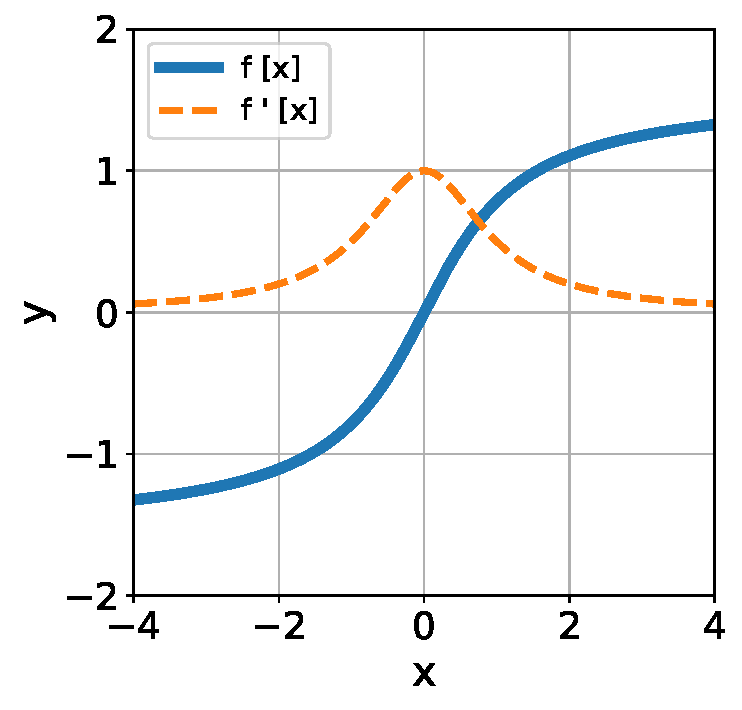
\includegraphics[width=0.65\textwidth]{figs/ann_arctan_function.pdf}

    \caption{Comportamento da função arco tangente.}
    \label{fig:ann_arctan_function}
\end{figure}


\linebreak
\newpage


\begin{definition}[Função \textit{Rectified Linear Unit} (ReLU)]
    Dada uma entrada $x$, a função ReLU pode ser definida como:

    \begin{equation}
        f[x] =  
        \begin{cases}
            0, & \text{se $x < 0$}\\
            x, & \text{se $x \geq 0$}
        \end{cases}
        \vspace{0.2cm}
        \label{eq:ann_relu_function}
    \end{equation}

    A derivada da função ReLU é:

    \begin{equation}
        f'[x] = u[x] = 
        \begin{cases}
            0, & \text{se $x < 0$}\\
            1, & \text{se $x \geq 0$}
        \end{cases}
        \vspace{0.2cm}
        \label{eq:ann_relu_function_dy}
    \end{equation}

\end{definition}

A Figura \ref{fig:ann_relu_function} exibe o comportamento da função ReLU \citep{nair2010rectified} acompanhado de sua primeira derivada.

\begin{figure}[H]
    \centering
    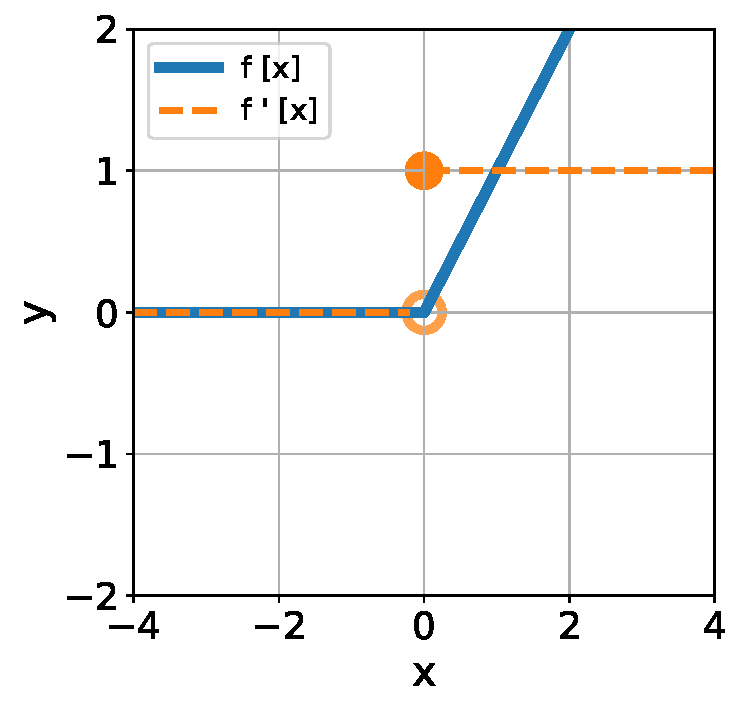
\includegraphics[width=0.65\textwidth]{figs/ann_relu_function.pdf}

    \caption{Comportamento da função ReLU.}
    \label{fig:ann_relu_function}
\end{figure}


\linebreak
\newpage


\begin{definition}[Função \textit{Leaky Rectified Linear Unit} (LReLU)]
    Dada uma entrada $x$, a função LReLU pode ser definida como:

    \begin{equation}
        f[x] = 
        \begin{cases}
            0.01 x, & \text{se $x < 0$}\\
            x, & \text{se $x \geq 0$}
        \end{cases}
        \vspace{0.2cm}
        \label{eq:ann_lrelu_function}
    \end{equation}

    A derivada da função LReLU é:

    \begin{equation}
        f'[x] = 
        \begin{cases}
            0.01, & \text{se $x < 0$}\\
            1, & \text{se $x \geq 0$}
        \end{cases}
        \vspace{0.2cm}
        \label{eq:ann_lrelu_function_dy}
    \end{equation}

\end{definition}

A Figura \ref{fig:ann_lrelu_function} exibe o comportamento da função LReLU \citep{maas2013rectifier} e sua primeira derivada.

\begin{figure}[H]
    \centering
    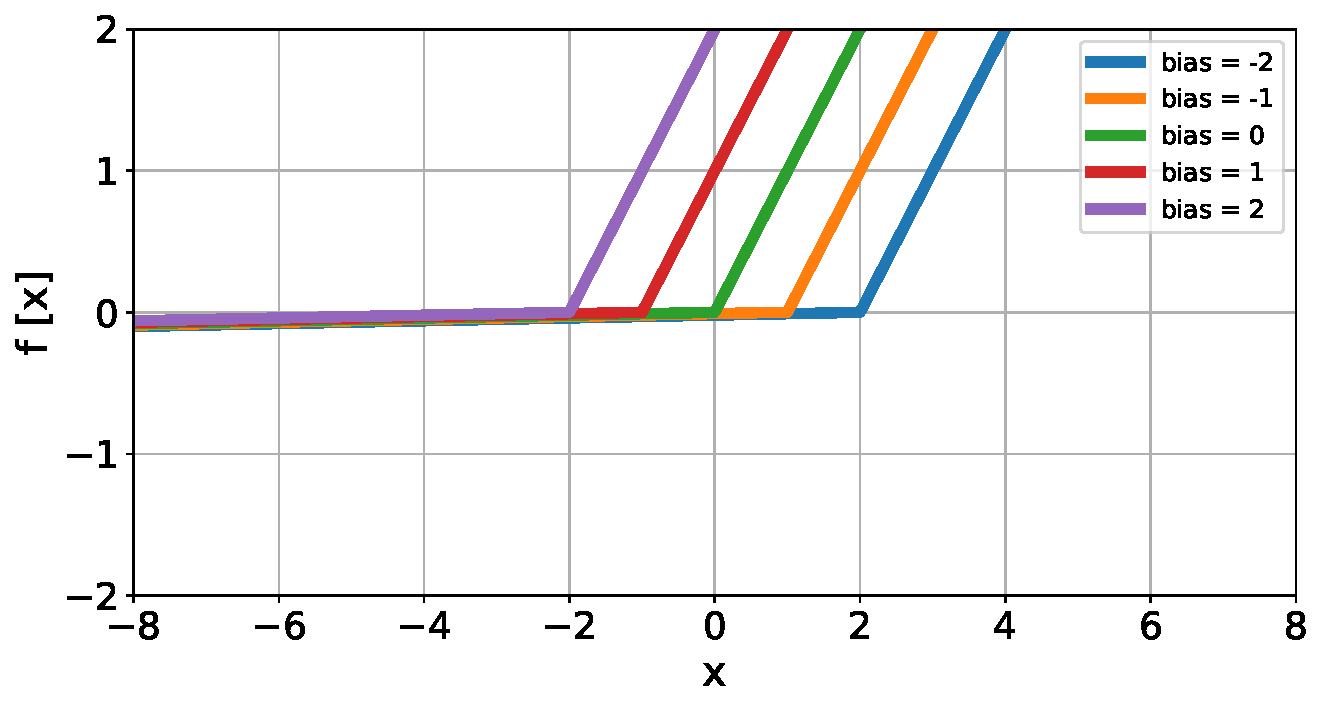
\includegraphics[width=0.65\textwidth]{figs/ann_lrelu_function.pdf}

    \caption{Comportamento da função LReLU.}
    \label{fig:ann_lrelu_function}
\end{figure}


\linebreak
\newpage


\begin{definition}[Função \textit{Inverse Square Root Rectified Linear Unit} (ISRLU)]
    Dada uma entrada $x$, a função ISRLU pode ser definida como:

    \begin{equation}
        f[x] = 
        \begin{cases}
            \dfrac{x}{\sqrt{1 + \alpha x^{2}}}, & \text{se $x < 0$}\\
            x, & \text{se $x \geq 0$}
        \end{cases}
        \vspace{0.2cm}
        \label{eq:ann_isrlu_function}
    \end{equation}

    A derivada da função ISRLU é:

    \begin{equation}
        f[x] = 
        \begin{cases}
            \left(\dfrac{1}{\sqrt{1 + \alpha x^{2}}}\right)^{3}, & \text{se $x < 0$}\\
            1, & \text{se $x \geq 0$}
        \end{cases}
        \vspace{0.2cm}
        \label{eq:ann_isrlu_function_dy}
    \end{equation}

\end{definition}

A Figura \ref{fig:ann_isrlu_function} exibe a função ISRLU \citep{carlile2017improving} junto à sua primeira derivada.

\begin{figure}[H]
    \centering
    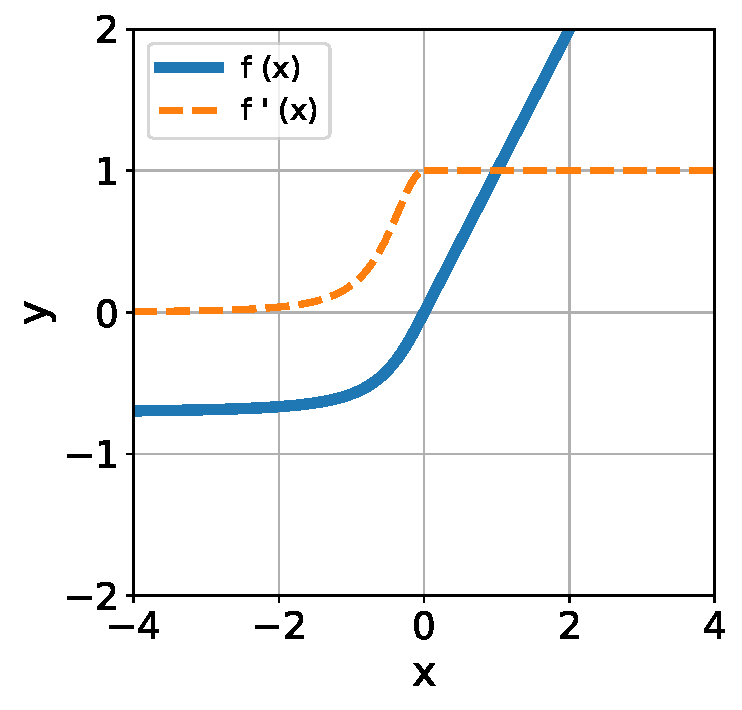
\includegraphics[width=0.65\textwidth]{figs/ann_isrlu_function.pdf}

    \caption{Comportamento da função ISRLU para $\alpha=1$ (em cima) e $\alpha=3$ (embaixo).}
    \label{fig:ann_isrlu_function}
\end{figure}


\linebreak
\newpage


%   ---------------------------------------
%   ----- Arquiteturas e Propriedades -----
%   ---------------------------------------
\section{Arquiteturas e Propriedades}
\label{sec:ann_arch_and_prop}

Uma Rede Neural Artificial (\textbf{ANN}, do inglês \textit{Artificial Neural Network}) é uma estrutura composta por neurônios interconectados distribuídos entre múltiplas camadas. Sua origem vem da ideia de imitar a função cerebral. Uma das características mais importantes das ANNs é a capacidade de aprender com ou sem supervisão (referências para análises comparativas), ou seja, as ANNs podem adotar uma abordagem de aprendizado supervisionado ou uma abordagem de aprendizado não supervisionada \citep{haykin1999neural}, dependendo da implementação do algoritmo de acordo com os objetivos do projeto.

\nomenclature{ANN}{\textit{Artificial Neural Network}}

Independentemente do tipo de rede neural artificial, os princípios básicos permanecem os mesmos; existem camadas de entrada, camadas ocultas e camadas de saída. Cada uma delas será explicada em mais detalhes posteriormente. Camadas ocultas são as principais responsáveis pelo aumento da demanda por poder de processamento, pois é onde residem os neurônios que realizam todo o processamento principal da rede.

Após uma primeira visão ingênua, talvez se imagine que, dado que os principais responsáveis pelo processamento são os neurônios localizados nas camadas intermediárias, o mais adequado seria aumentar sumariamente o número de neurônios para que isso produzisse um agressivo ganho de desempenho na atividade realizada pela rede; contudo, tal decisão seria, muito provavelmente, bastante equivocada e, sem dúvidas, nem um pouco parcimoniosa. Para se obter melhores resultados, portanto, é preciso estudar melhor sobre o funcionamento dos elementos que compõem toda a rede, além de explorar e analisar diferentes arquiteturas que podem ser mais propícias a responder melhor em certos ambientes específicos.

O impacto causado pelas redes neurais artificiais se intensificou drasticamente a partir da criação do Perceptron Multicamadas (\textbf{MLP}, \textit{Multilayer Perceptron}), que consiste em uma classe de redes de em que a informação é propagada apenas em uma direção, sendo enviada para a frente da rede. A estrutura de um MLP é composta por ao menos duas camadas intermediárias de neurônios, tal como pode ser visto pela Figura \ref{fig:ann_mlp}, o que permite que, em vez de ser projetado um único hiperplano para separar o hiperespaço de amostras a serem classificadas, passe a ser possível obter modelos bem mais flexíveis quanto a essas regiões de fronteira de separação.

\nomenclature{MLP}{\textit{Multilayer Perceptron}}

\begin{figure}[H]
    \centering
    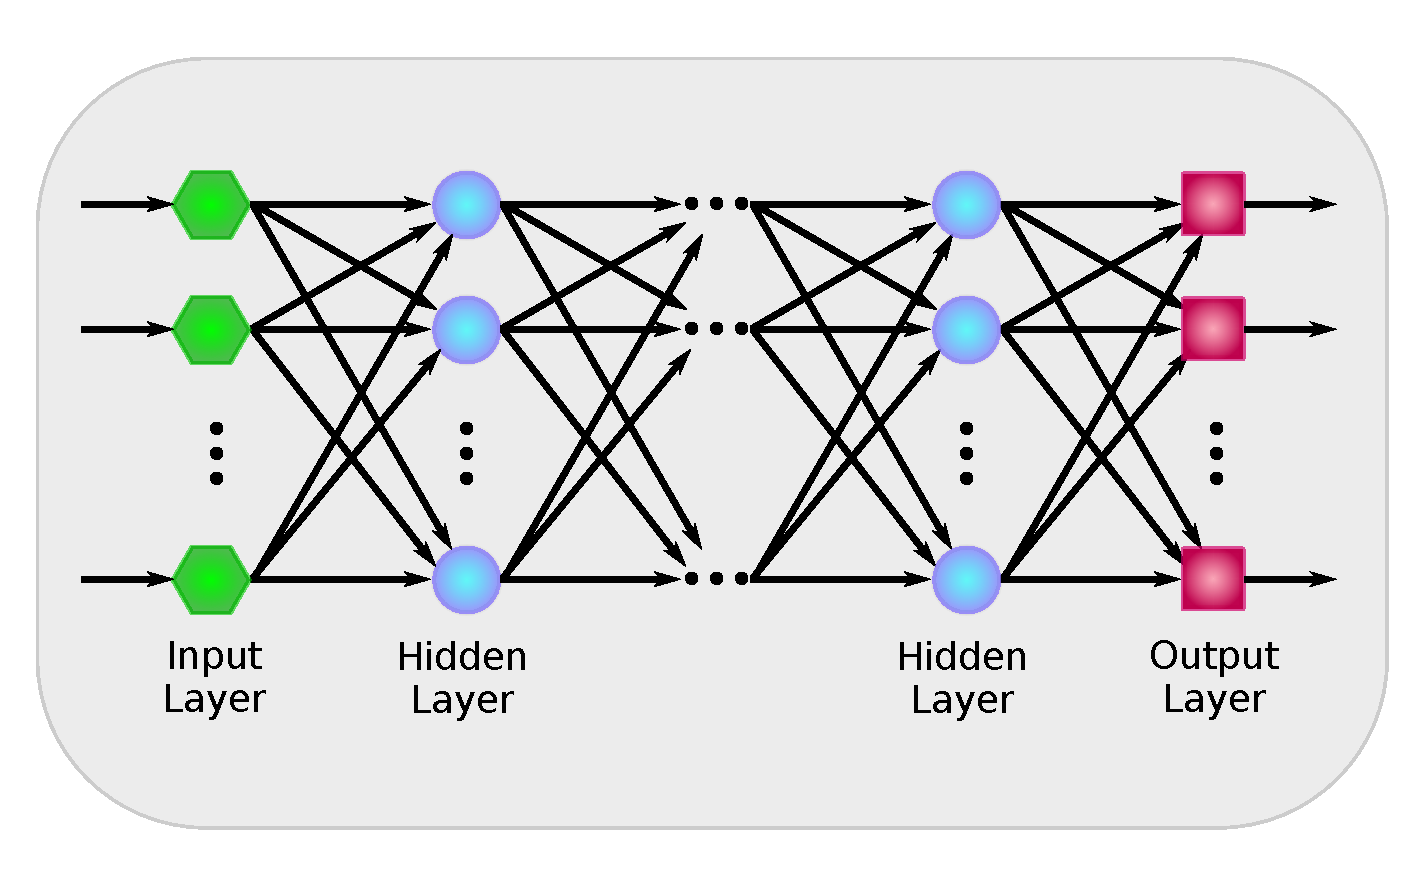
\includegraphics[width=0.8\textwidth]{figs/ann_mlp.pdf}
    \caption{Representação esquemática e genérica de um MLP.}
    \label{fig:ann_mlp}
\end{figure}

Já de longa data, os resultados obtidos levavam pesquisadores e desenvolvedores a acreditar que sua estrutura possuía características intrínsecas de alta capacidade de aproximação de modelos e, embora ainda não tivessem sido matematicamente provadas tais características, sua exploração por parte de diversos pesquisadores resultou em muitos importantes avanços na área. Ao fim da década de 1980 foram publicados trabalhos que efetuavam tal prova matemática em relação à sua capacidade de aproximação \citep{cybenko1989approximation, hornik1989multilayer}, embora tenha sido feita com base em funções sigmoidais. Pouco tempo depois foi publicado um trabalho que provava que, na verdade, essa capacidade de aproximação não era oriunda da função de ativação, mas, em vez disso, era advinda da própria estrutura do MLP, cujo fluxo de informação é direcionado para frente \citep{HORNIK1991251}.

Em 2017 foi provado que o Teorema da Aproximação Universal se aplica a redes profundas que utilizem funções de ativação do tipo ReLU quando respeitada a condição de que haja uma largura\footnote{Neste contexto, a largura da rede se refere apenas ao número de camadas intermediárias que a rede em questão possui, independentemente da quantidade de neurônios que cada uma possua ou da forma como os neurônios efetuem a comunicação entre camadas distintas.} mínima de $n+4$ camadas com o objetivo de se aproximar quaisquer funções que sejam Lebesgue integráveis \citep{royden1988real}. Finalmente, ainda no mesmo ano, foi provada essa capacidade de aproximação universal para qualquer função convexa contínua e, desta vez, necessitando apenas de $n+1$ camadas \citep{hanin2017universal}.




%   ---------------------------
%   ----- Backpropagation -----
%   ---------------------------
\section{Backpropagation}
\label{sec:ann_backpropagation}



%   -----------------------------------------------
%   ----- Aplicação aos Problemas Mencionados -----
%   -----------------------------------------------
\section{Aplicação aos Problemas Mencionados}
\label{sec:ann_application_mentioned_problem}



%   ---------------------------
%   ----- Redes Profundas -----
%   ---------------------------
\section{Redes Profundas}
\label{sec:ann_deep_networks}



%   ----- Neurônios -----
\subsection{Neurônios}
\label{subsec:ann_neurons}



%   ----- Treinamento -----
\subsection{Treinamento}
\label{subsec:ann_training}



%   ----- Inicialização -----
\subsection{Inicialização}
\label{subsec:ann_inicialization}
